\section{ПРОЕКТИРОВАНИЕ}
    \subsection{Концептуальная модель обработки сообщений}
    Главной целью при разработке новой архитектуры чат-бот ставилась возможность
    разбиение процесса обработки на основные этапы, которые можно было бы
    распределить между независимыми классами, с единственной ответственностью и
    высоким потенциалом переиспользования.
    Процесс обработки сообщения можно разделить на следующие этапы:
    \begin{enumerate}
        \item Получение сообщения через интерфейс (IMAP, LongPoll ВКонтакте, 
        telegram-api, http-POST)
        \item Извлечение необходимых полей из инородной структуры данных и 
        преобразование в объект-сообщение внутреннего типа
        \item Классификация сообщения
        \item Формирование ответов на сообщение
        \item Отправка ответов обратно через интерфейс библиотеки пользователю
        \item Сохранение всех сообщений в базу
        \item Выполнение дополнительных действий (запрос обратной связи от
        пользователя, логгирование и прочее)
    \end{enumerate}

    Таким образом, за каждый из этапов обработки сообщения отвечать будет свой 
    отдельный объект, притом, на этапе 3 и 4 абсолютно не важно, по какому 
    каналу было получено сообщение, равно как на этапе 5 и 6. Этапы 1, 2 и 5, 
    наоборот, направлены исключительно на адаптацию к внешним API и библиотекам.
    Для их реализации будет применен паттерн "Адаптер". Для реализации этапов
    6 и 7 будет использован паттерн "Наблюдатель".\cite{design.patterns}

    
    \subsection{Описание участников обработки сообщений}
    \subsubsection*{ApiWorker}
    Класс-адаптер ответственный за первый этап -- \inlinecode{ApiWorker}.
    Его ответственность -- постоянная обработка входящих сообщений от 
    пользователя и исходящих сообщений от оператора и бота, используя библиотеки
    для работы с каналами. Обладает одним методом, который запускает процесс 
    получения новых сообщений. Его код представлен на листинге ниже.

    \begin{figure}[!h]
        \centering
        \lstinputlisting[language=Python]{snippets/api_worker.py}
        \caption{Код класса ApiWorker}
        \label{fig:api_worker}
    \end{figure}

    \subsubsection*{ApiWrapper}
    Ещё один класс-адаптер, ответственный за превращение полученного сообщения 
    во объект-контейнер MessageData, обратное превращение перед отправкой
    сообщения пользователю и непосредственную отправку.
    Его интерфейс выглядит следующим образом:

    \begin{figure}[!h]
        \centering
        \lstinputlisting[language=Python]{snippets/api_wrapper.py}
        \caption{Код класса ApiWrapper}
        \label{fig:api_wrapper}
    \end{figure}
    
    Метод \inlinecode{send_answers} отправляет все ответы из списка, дополняя их
    необходимой информацией от сервера текущего канала. 
    Метод \inlinecode{send_message} отправляет одно отельное сообщения по текущему каналу,
    возвращает то же сообщение, но дополненное информацией от сервера: реальным временем
    отправки, идентификатором, который сервер канала обозначил это сообщение и так далее.

    \subsubsection*{Notifier}
    Если событие, произошедшее во время работы объекта ApiWorker необходимо
    зарегистрировать, то для этого будет использован один из классов,
    реализующих интерфейс Notifier.
    Схема уведомлений реализована в соответствии с паттерном Издатель-подписчик.
    Каждый ApiWorker обладает набором Notifier-подписчиков, каждому из которых
    отправляется уведомление о событии \inlinecode{Notifier.notify}.
    Уведомления могут понадобиться для создания записи в базе о новых сообщениях,
    или для отправки логов работы в мессенджер разработчика или заказчика.

    \subsubsection*{MessageHandler}
    Все действия между получением сообщения в \inlinecode{ApiWorker.run} и отправкой ответов
    в \inlinecode{ApiWrapper.send_answers} и сохранением в базу будет скрывать в себе метод
    \inlinecode{MessageHandler.handle}. Для входящих сообщений от пользователя обрабатывать
    сообщения будет IncomingHandler, для исходящих от оператора и бота -- OutgoingHandler.
    Интерфейс класса MessageHandler представлен в листинге ниже.

    \begin{figure}[!h]
        \centering
        \lstinputlisting[language=Python]{snippets/message_handler.py}
        \caption{Код класса MessageHandler}
        \label{fig:message_handler}
    \end{figure}

    Метод \inlinecode{MessageHandler.notify} здесь исполняет отправку всех уведомлений,
    которые были переданы ему.

    Обработчик входящих сообщений, IncomingHandler, также должен вырабатывать 
    ответ к входящему сообщению. Эту задачу он делегирует другому 
    классу -- Scenarist. Дополнительно IncomingHandler может исполнять некоторые
    действия, в зависимости от выбранного сценария.
    Общий вид класса IncomingHandler представлен на листинге ниже.

    \begin{figure}[!h]
        \centering
        \lstinputlisting[language=Python]{snippets/incoming_handler.py}
        \caption{Код класса IncomingHandler}
        \label{fig:incoming_handler}
    \end{figure}

    \subsubsection*{Прочие компоненты}
    AbstractScenarist -- интерфейс сценариста, обладает только одним методом:\\
    \inlinecode{AbstractScenarist.run_scenario}, который при реализации, должен
    будет выработать нужную реакцию (ResponseData) на входящее сообщение с
    набором нужных ответов (Answer) и действий (Action).

    Задачу предсказания сценарист делегирует классификатору (Classifier),
    обладающему единственным методом \inlinecode{Classifier.predict}, который
    возвращает объект Prediction с набором меток обнаруженных в тексте сообщения
    классов. По этим меткам и будет составлена ResponseData внутри сценариста.

    Работа с базой данных будет инкапсулирована в классе DataBaseProvider.

    \subsection{Диаграммы}
    Теперь, когда мы выполнили описание всех участников обработки сообщений,
    можем для большей наглядности представить их на диаграмме классов.
    Сам процесс обработки одного сообщения изобразим на диаграмме процессов.

    Диаграмма классов представлена на рисунке ниже.
    \begin{figure}[!h]
        \centering
        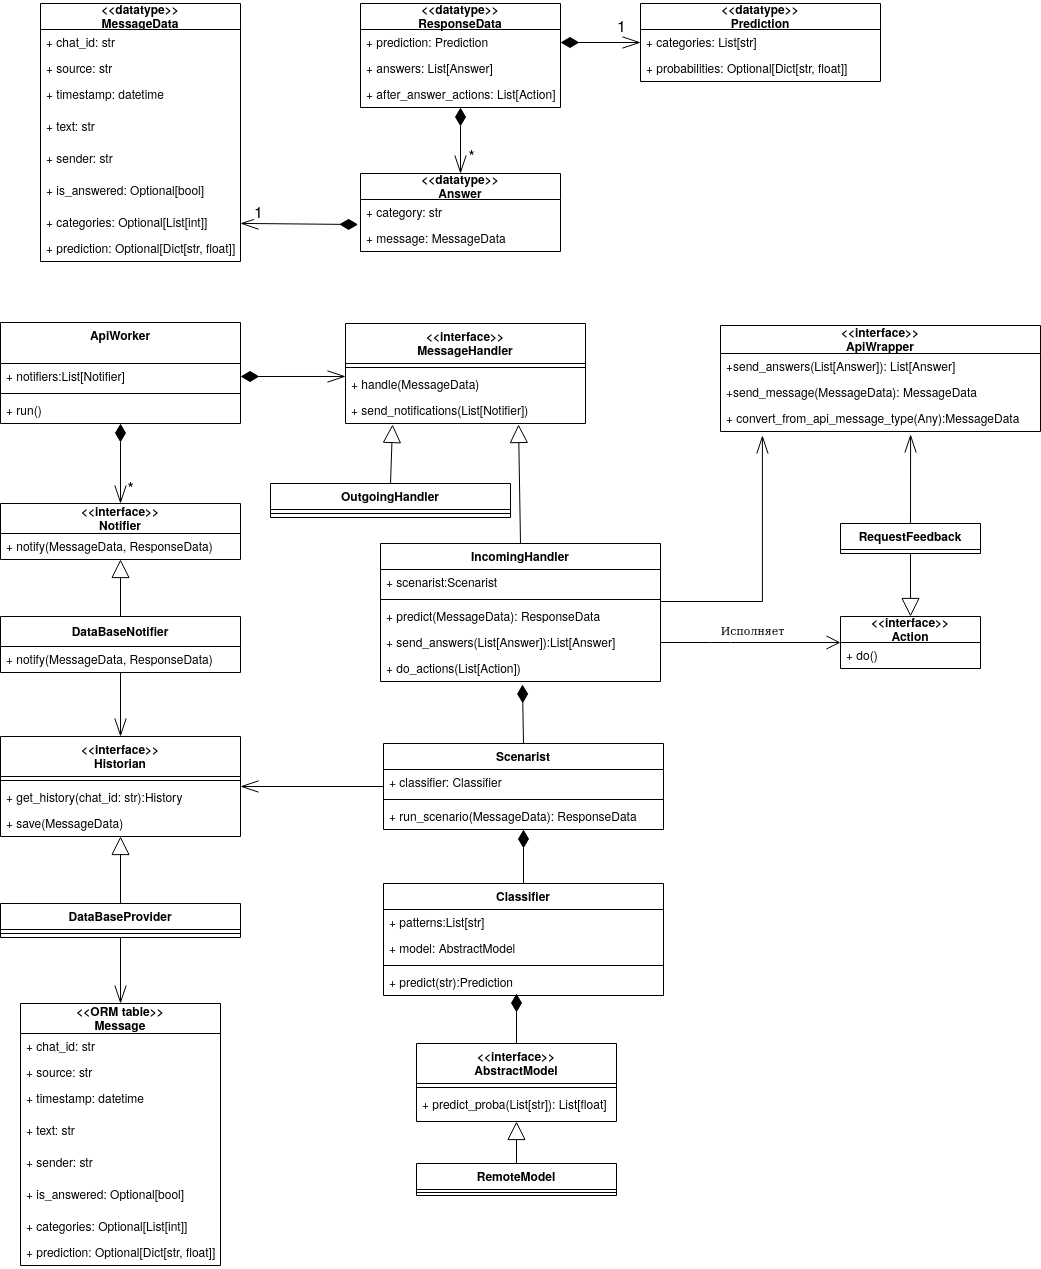
\includegraphics[width=\linewidth]{static/ClassDiagram.png}
        \caption{Диаграмма классов проекта}
        \label{fig:class-diagram}
    \end{figure}

    % Диаграмма процесса обработки сообщения представлена на рисунке ниже.
    % \begin{figure}[!h]
    %     \centering
    %     % TODO Диаграмма процесса
    %     % \includegraphics[width=\linewidth]{}
    %     \caption{Диаграмма процесса обработки сообщения}
    %     \label{fig:func-schema-before}
    % \end{figure}

    \subsection*{Вывод по главе 2}
    В этой главе мы сформулировали основную концепцию нашей будущей системы, 
    описали основные её сущности и способы их взаимодействия. Мы в коде описали 
    сигнатуры их публичных методов базовых классов.
    % , и изобразили основные классы и процессы на диаграммах.
    Теперь, мы можем приступать к их реализации в каждом конкретном канале.
